\subsection{Replication on ERP CORE}
Table~\ref{tab:erpcore} and Fig.~\ref{fig:erpcore} report the pre-stimulus statistic for the five ERP CORE paradigms. Under both scalings that use no post-stimulus sample, every paradigm sits inside its permutation null in both regimes. Under per-epoch z-scoring, the across-participant statistic exceeds its null in the paradigms with a sustained one-signed condition difference: N170 at 0.573 ($p=0.0040$), P3 at 0.695 ($p=0.0005$), and N400 at 0.715 ($p=0.0005$) with 2000 permutations, or 0.008, 0.0025, and 0.0025 after Holm adjustment over the five paradigms. The post-stimulus variant gives 0.582, 0.703, and 0.724. The lateralized N2pc, whose condition difference reverses sign across hemispheres, also leaks across participants (0.597, $p=0.005$), because each channel's epoch mean carries its own signed contrast and the decoder reads the pattern across channels. One N2pc participant has no retained trial in one condition and is excluded from that paradigm.


Within participants, on single trials, the mechanism is present at the smaller magnitude the averaging law predicts for $k=1$. Under per-epoch z-scoring the N400 statistic is 0.537 ($t$-test $p=5.2\times10^{-8}$, 36 of 40 participants above 0.5), while N170 and P3 give 0.515 ($p=0.084$) and 0.504 ($p=0.052$). The post-stimulus variant reaches significance in all three (N170 0.520, $p=0.024$, P3 0.507, $p=0.018$, and N400 0.544, $p=1.3\times10^{-8}$).

Scaling the participant average directly, the order of the SHAPE pipeline, yields the same pattern (N170 0.569, P3 0.595, N400 0.717, each $p\le0.01$), and a decoder fed $-m/\hat\sigma$ of each average reaches 0.603, 0.630, and 0.790.

\begin{table*}[t]
\centering
\caption{ERP CORE: mean pre-stimulus decoding accuracy ($-200$ to $0$~ms, 15.6~ms bins), two classes, chance 0.5, 40 participants per paradigm. Across participants: trials scaled, then averaged; $p$ from 200 label permutations. Within participants: single trials; mean [95\% CI] and one-sample $t$-test $p$ against 0.5.}
\label{tab:erpcore}
\begin{tabular}{llcccc}
\toprule
Paradigm & Regime & \texttt{none} & \texttt{pre\_sd} & \texttt{epoch\_z} & \texttt{post\_z} \\
\midrule
\multirow{2}{*}{N170} & across & 0.488 ($p=0.726$) & 0.492 ($p=0.567$) & 0.573 ($p=0.005$) & 0.582 ($p=0.010$) \\
 & within & 0.508 ($p=0.36$) & 0.505 ($p=0.53$) & 0.515 ($p=0.084$) & 0.520 ($p=0.024$) \\
\multirow{2}{*}{P3} & across & 0.520 ($p=0.234$) & 0.524 ($p=0.169$) & 0.695 ($p=0.005$) & 0.703 ($p=0.005$) \\
 & within & 0.500 ($p=0.84$) & 0.499 ($p=0.32$) & 0.504 ($p=0.052$) & 0.507 ($p=0.018$) \\
\multirow{2}{*}{N400} & across & 0.488 ($p=0.701$) & 0.486 ($p=0.687$) & 0.715 ($p=0.005$) & 0.724 ($p=0.005$) \\
 & within & 0.499 ($p=0.71$) & 0.501 ($p=0.77$) & 0.537 ($p=5.2e-08$) & 0.544 ($p=1.3e-08$) \\
\multirow{2}{*}{N2pc} & across & 0.502 ($p=0.478$) & 0.483 ($p=0.761$) & 0.597 ($p=0.005$) & 0.597 ($p=0.005$) \\
 & within & 0.504 ($p=0.14$) & 0.504 ($p=0.095$) & 0.510 ($p=0.0084$) & 0.511 ($p=0.017$) \\
\multirow{2}{*}{MMN} & across & 0.537 ($p=0.070$) & 0.524 ($p=0.174$) & 0.553 ($p=0.045$) & 0.592 ($p=0.025$) \\
 & within & 0.500 ($p=0.66$) & 0.500 ($p=0.3$) & 0.499 ($p=0.0014$) & 0.499 ($p=0.011$) \\
\bottomrule
\end{tabular}
\end{table*}


\begin{figure*}[t]
\centering
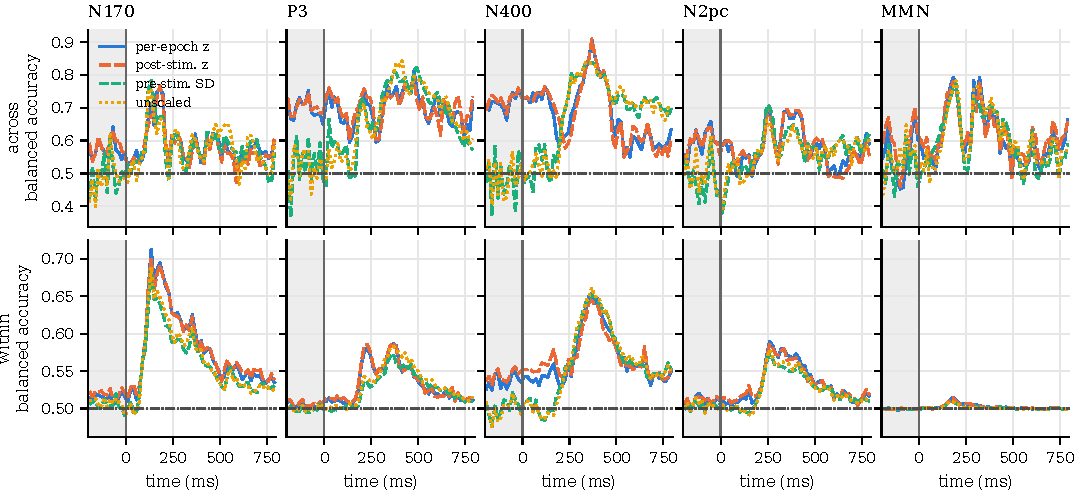
\includegraphics[width=\textwidth]{figures/fig_erpcore.pdf}
\caption{ERP CORE time-resolved decoding of the 28-channel pattern in 15.6~ms bins, chance 0.5 (dash-dot), pre-stimulus interval shaded. Top: across participants (trials scaled, then averaged). Bottom: within participants (single trials, mean over participants). Under per-epoch and post-stimulus z-scoring the curves rise above chance before onset.}
\label{fig:erpcore}
\end{figure*}
